\documentclass[11pt,a4paper,onecolumn]{article}

\usepackage{latexsym}      % needed math symbols
\usepackage{hyperref}
\hypersetup{
 colorlinks=true,
 citecolor=blue,
 linkcolor=blue,
 urlcolor=blue,
 pdfpagemode=UseNone,
 pdfstartview=FitH}
\usepackage{graphicx}      % for importing eps figures
\usepackage{amsmath}       % for advanced math symbols
\usepackage[affil-it]{authblk} 			% found in preprint bundle package, http://ctan.org/pkg/preprint
\usepackage[margin=1.97cm]{geometry} % paper and margin formats as set by SPP
\usepackage[english]{babel}
\usepackage{booktabs}
\usepackage{textcomp}

\parindent 0.5cm    % paragraphs indent

% authblk style
\renewcommand\Authfont{\large}
\renewcommand\Affilfont{\normalsize	\itshape}
\setlength{\affilsep}{5pt}

% for abstract style
\makeatletter
\newbox\abstract@box
\renewenvironment{abstract}
  {\global\setbox\abstract@box=\vbox\bgroup
     \hsize=\textwidth\linewidth=\textwidth
    \small
    \quotation}
  {\endquotation\egroup}
\expandafter\def\expandafter\@maketitle\expandafter{\@maketitle
  \ifvoid\abstract@box\else\unvbox\abstract@box\if@twocolumn\vskip1.5em\fi\fi}
\makeatother
\providecommand{\keywords}[1]{\noindent \mdseries{{Keywords:}} #1}
\providecommand{\DOI}[1]{\vspace{1\baselineskip}}
\providecommand{\dateline}[1]{\vspace*{-1\baselineskip}\normalsize #1\vspace*{-1.5\baselineskip}}

% for the figure and tables, captions
\usepackage{booktabs}
\usepackage{dcolumn}
\newcolumntype{d}[1]{D{.}{.}{#1}}

\usepackage{caption}
\captionsetup[table]{position=above, font={rm,small}, labelfont=bf, labelsep=period}
\captionsetup[figure]{font={rm,small}, labelfont=bf, labelsep=period}

% for citations formatting style
\usepackage[numbers,square,sort&compress]{natbib}
\setlength\bibsep{1pt}

% other packages and macros
\usepackage{float}
\usepackage{bm}
\renewcommand{\vec}[1]{\text{\bfseries #1}}

% turn off hyphenation
\hyphenchar\font=-1

% page numbering
\pagenumbering{arabic}

% Font
\usepackage{mathpazo}

\begin{document}

%--------------------------------------------------------------------------
%  fill in the paper's title, author(s), and corresponding institutions
%--------------------------------------------------------------------------

\title{\textbf{Serotonin induces a \textsc{down} state across the anesthetized mouse brain}}
\author{Rosa Großmann\textsuperscript{1}, Jorge F. Mejias\textsuperscript{2}, International Brain Laboratory, Zachary F. Mainen\textsuperscript{3} \& Guido T. Meijer\textsuperscript{3,4}}
\affil{\textsuperscript{1}Max Planck Institute for Human Cognitive and Brain Science, Leipzig, Germany\newline
\textsuperscript{2} Cognitive and Systems Neuroscience Group, Swammerdam Institute for Life Sciences, University of Amsterdam, Amsterdam, The Netherlands\newline
\textsuperscript{3}Champalimaud Foundation, Lisbon, Portugal\newline
\textsuperscript{4}Donders Centre for Neuroscience, Radboud University Nijmegen, The Netherlands}

\date{}

\begin{abstract}
\noindent
%---------------------------------------------------------------------------
%               Include abstract and keywords here
%---------------------------------------------------------------------------
Serotonergic neurons in the dorsal raphe nucleus (DRN) project extensively throughout the forebrain, yet their influence on global network states remains controversial. Serotonin is implicated in regulating slow-oscillations, so-called UP and DOWN states, which occur during sleep and light anesthesia. While optogenetic fMRI suggests that serotonin (5-HT) suppresses brain-wide activity, classical electrical stimulation studies report the induction of cortical UP states. To resolve this discrepancy, we combined optogenetic 5-HT stimulation with large-scale Neuropixel recordings across the forebrain of lightly anesthetized mice. We demonstrate that selective 5-HT release consistently induces DOWN states across the cortex and striatum, while leaving midbrain dynamics largely unaffected. Using a multi-area computational model constrained by biologically plausible connectivity, we show that these transitions are not solely dependent on direct DRN innervation. Instead, 5-HT-induced state transitions propagate to remote cortical regions via network-level interactions.

\DOI{} % do not delete this line
\end{abstract}

\maketitle
\thispagestyle{empty}

%---------------------------------------------------------------------------
%               the main text of your paper begins here
%---------------------------------------------------------------------------
\section*{Introduction}

Serotonin (5-HT) is a neuromodulator which plays a crucial role in many brain functions and modulates neural activity in various ways \cite{celadaSerotoninModulationCortical2013}. One of the activity patterns in the brain which is modulated by serotonin are slow oscillations, with alternating states of high and low activity, also referred to as UP and DOWN states. Slow oscillations appear during anaesthesia and slow-wave sleep and are important for learning, memory consolidation and plasticity \cite{neskeSlowOscillationCortical2015}, they are thought to be the default emergent activity of neural networks \cite{sanchez-vivesShapingDefaultActivity2017,neskeSlowOscillationCortical2015}. Altough it is clear that serotonin affects slow oscillations, different studies arrive at conflicting conclusions as to the directionality of its effect.

It was shown that inceasing tonic levels of serotonin by administering MDMA supresses slow oscillations in anaesthetised mice. Furthermore, bath application of 5-HT to acute brain slices completely abolishes slow oscillations \cite{defilippoSomatostatinInterneuronsActivated2021}. Besides these slow tonic increases in serotonin, also transient pulses of 5-HT suppress neural activity across the brain, as measured with fMRI \cite{hamadaOptogeneticActivationDorsal2022,grandjeanBrainwideFunctionalMap2019}. Altough these studies suggest that serotonin induces a DOWN state, they lack the temporal precision to directly establish this. Another piece of evidence which supports the notion that serotonin should induce a DOWN state is that 5-HT stimulation suppresses hippocampal sharp wave ripples \cite{kandilakisOppositeSerotonergicModulation2025,meijerSerotoninDrivesChoiceindependent2025}. Since sharp wave ripples occur during UP states it is likely that serotonin transitions the neural network into a DOWN state. This is, however, only indirect evidence. In contrast to the previous findings, one study showed that electrical stimulation of the dorsal raphe nucleus (DRN) in rats induces an UP state in frontal cortex \cite{puigSerotoninModulatesFastSpiking2010}. To our knowledge, this is the only study which investigated the direct effect of a transient increase of serotonin on UP-DOWN dynamics with high temporal resolution. Their findings, however, are in direct conflict with a body of literature which indicates that serotonin suppresses neural activity and transitions the network into a DOWN state. Serotonin's effect on UP-DOWN state dynamics under anesthesia is therefore still a topic for debate.

To shed light on this issue, we stimulated serotonin by optogenetically activating DRN neurons in the anesthetized mouse while recording single cell spiking activity across the brain with Neuropixel probes. We found that 5-HT stimulation rapidly induced a DOWN state in cortex, amygdala, striatum, hippocampus, thalamus, but not the midbrain. To investigate the underlying mechanism of this effect we modelled UP-DOWN state dynamics with a firing rate model with realistic inter-area connectivity which replicates the experimental data \cite{mejiasIrregularDynamicsCortical2010,jercogUPDOWNCorticalDynamics2017}. 

\begin{figure}[t]
    \centering
    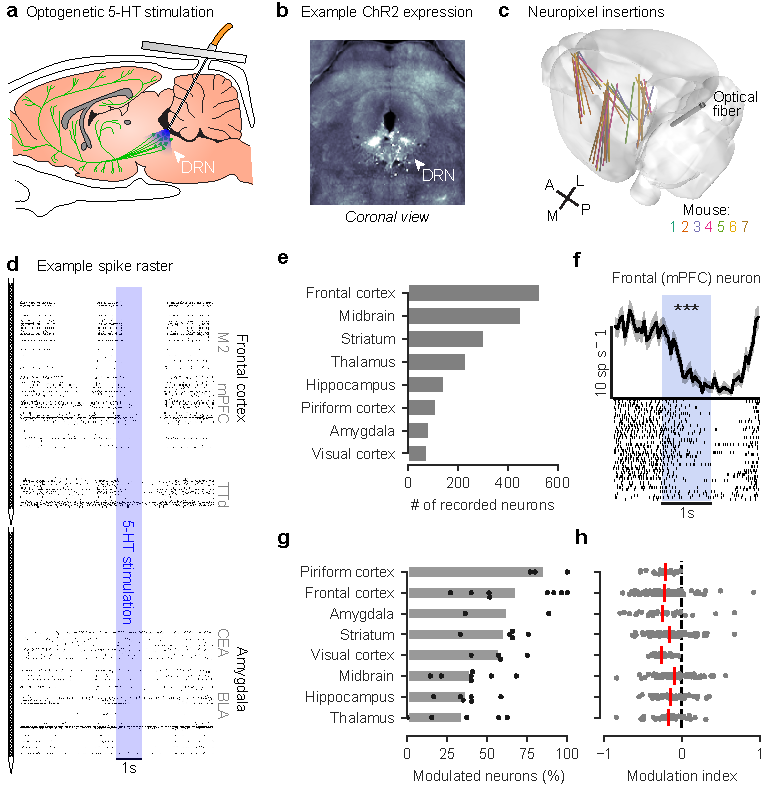
\includegraphics[width=1\textwidth]{img/recordings_overview.pdf}
    \caption{Acute Neuropixel recordings while optogenetically stimulating serotonin release. (a) Saggital cartoon drawing of serotonergic neurons in the DRN projecting throughout the brain (green). An optical fiber is positioned directly above the DRN through the cerebellum through which the 5-HT neurons can be activated with blue light. (b) A coronal histological section of the DRN showing expression of channelrhodopsin. (c) A coronal histological section showing the fluorescent tract of a Di-I coated Neuropixel insertion. (d) Neuropixel insertion trajectories, aligned to the Allen Brain reference atlas, across all seven mice. Typically seven insertions were made per mouse, color of each insertion indicates mouse identity.}
    \label{fig:recordings}
\end{figure}

\section*{Results}
We performed acute Neuropixel recordings across the mouse brain while the animal was under light anesthesia. Over four consecutive recording days, seven Neuropixel insertions were made targeting frontal cortex, visual cortex, amygdala, striatum, hippocampus, thalamus, and the midbrain. Serotonin was stimulated by activating serotonergic neurons in the DRN optogenetically during Neuropixel recordings in the forebrain (Fig. \ref{fig:recordings}).

Cortical UP-DOWN states were clearly visible under anesthesia as periods of 1-2s of neural activity interspersed with periods of silence (Fig. \ref{fig:ephys}a). Based on visual inspection of the spike raster plots, 5-HT stimulation appeared to coincide with a DOWN state. To investigate this, first we asked what the effect of serotonin stimulation was on the activity of single neurons. Peri-stimulus time histograms of single neurons, conditioned on the start of the 5-HT stimulation, consistently showed that single neuron spiking activity was decreased (example neuron in Fig. \ref{fig:recordings}b). In all recorded brain regions we found a large fraction of neurons that were significantly modulated by serotonin stimulation (30-60\%; ZETA-test \cite{montijn_parameter-free_2021}, \emph{p} $<$ 0.05; Fig. \ref{fig:ephys}c). A large majority of single neurons were suppressed by 5-HT stimulation as quantified by their modulation index, which was predominantly $<$ 0. The mean modulation index over neurons per brain region was negative indicating that all recorded regions were suppressed by serotonin stimulation (Fig. \ref{fig:ephys}d). 

To directly investigate whether serotonin stimulation induced a DOWN state we quantified UP and DOWN states with a two-state Hidden Markov Model (HMM) which was fit to spike rates conditioned to the start of the 5-HT stimulation (Fig. \ref{fig:ephys}e,f). We found that serotonin stimulation strongly and rapidly induced a DOWN state in the frontal cortex, this effect scaled with the stimulation frequency of the optogenetic stimulation (Fig. \ref{fig:ephys}g). Performing the analysis across all recorded brain regions we found that serotonin strongly induced a DOWN state in the frontal cortex and striatum, to a lesser extend in the amygdala, visual cortex, hippocampus, and thalamus, and not at all in the midbrain (Fig. \ref{fig:ephys}h).

\begin{figure}[!t]
    \centering
    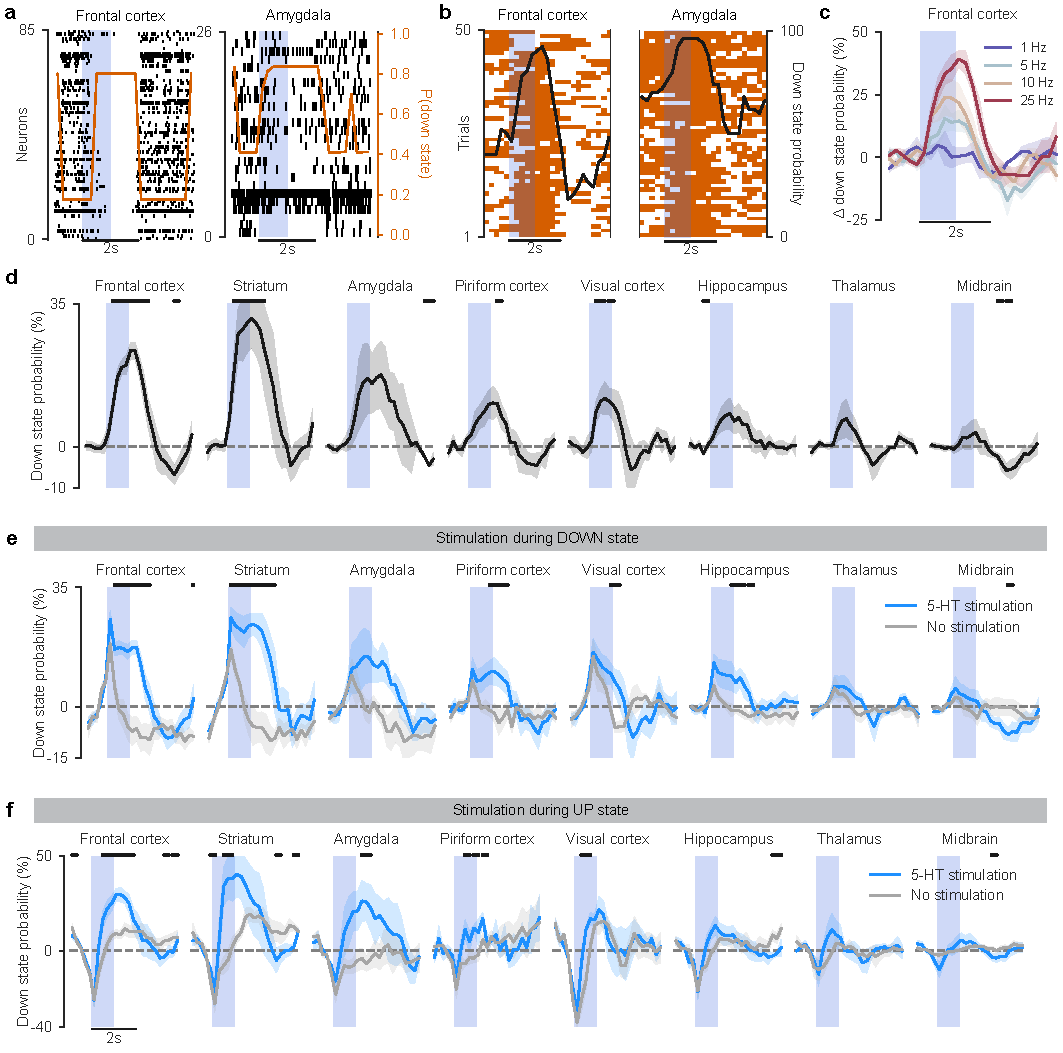
\includegraphics[width=1\textwidth]{img/ephys_updown_states.pdf}
    \caption{Serotonin induces a DOWN state under anesthesia. (a) An example spike raster plot of 10s of spiking activity recorded on two Neuropixel probes simultaneously. Recorded brain regions are indicated on the right of the raster at their approximate depths. The time of the optogenetic 5-HT stimulation is indicated by the blue bar (25 Hz, 10 ms pulses). (b) Peri-stimulus time histogram of an example neuron from the frontal cortex. The bottom shows the spike raster in which each row is a repetition of 1s 25 Hz stimulation. The top shows the mean spiking rate binned in 50 ms bins with a 25 ms Gaussian smoothing kernel. *** \emph{p} $<$ 0.001, ZETA-test. (c) Percentage of significantly modulated neurons (ZETA-test, \emph{p} $<$ 0.05) per brain region, calculated per recording session. Black dots are sessions, grey bars means over sessions. (d) Modulation index per neuron, negative values indicate the neuron is inhibited by 5-HT and positive values indicate excitation. Each grey dot is a single neuron, vertical red bars are the mean over neurons per brain region. (e) An example peri-stimulus raster plots of spike times (black ticks, each row is a neuron), aligned to the onset of 5-HT stimulation (blue vertical bar). The orange line indicates the posterior probability of a DOWN state as determined by a two-state HMM. On the left an example from the frontal cortex is shown and on the right an example from the amygdala. (f) A peri-stimulus heatmap over trials of when the HMM determined there most likely was a DOWN state (orange). The black line is the mean posterior probability of a DOWN state over trials per time bin. (g) A peri-stimulus plot of the change in DOWN state probability compared to baseline (-1 to 0s) averaged over mice (n = 5, mean $\pm$ sem). Plotted separately, indicated by color, are different stimulation frequencies. (h) Peri-stimulus plots for all recorded high-level brain regions of the change in DOWN state probability over baseline for 25 Hz serotonin stimulation.} 
    \label{fig:ephys}
\end{figure}

We implemented a dynamic bistable firing rate model to investigate the mechanism by which serotonin stimulation results in the induction of DOWN states. The model simulates a simplified network of the mouse brain, following biological realistic inter-area connectivity. Each brain area was modelled using a local excitatory-inhibitory (EI) circuit consisting of one E, one I population, and a mechanism controlling for adaptation (A) of the excitatory population  \cite{jercogUPDOWNCorticalDynamics2017} (Fig. \ref{fig:model_updown}a). To introduce biologically plausible connectivity between the modelled brain regions, the projection strength between them was pulled from the Mouse Connectivity Atlas of the Allen Brain Atlas, together with the projection strength of the dorsal raphe nucleus to these regions (Fig \ref{fig:model_updown}b. The model was able to reproduce slow-wave oscillations which mimicked closely the UP and DOWN states observed in the neural data (Fig. \ref{fig:model_updown}c). The frequency of modelled UP and DOWN states was around 0.5-1 Hz which closely matched the frequency observed in the brain. 

\begin{figure}[t]
    \centering
    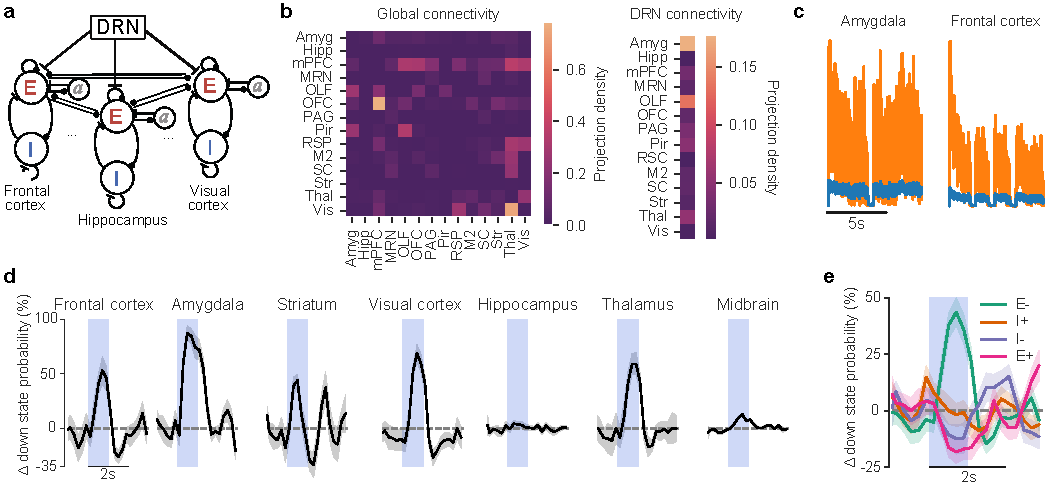
\includegraphics[width=1\textwidth]{img/Results/Fig3_model_GM.pdf}
    \caption{Simulation of UP-DOWN state dynamics by a bistable firing rate model. (a) A global circuit model of interconnected brain regions which receive input from the dorsal raphe nucleus (DRN). (b) Connectivity matrix for the global circuit and DRN projections. (c) The modelled activity recapitulated UP-DOWN state dynamics in brain regions which also show these dynamics in the brain; e.g. the frontal cortex. (d) Modelled serotonin stimulation induced a DOWN state in several brain regions. The change in DOWN state probability versus baseline (-1 to 0s) is plotted per brain region. (e) DOWN states were induced by inhibiting the excitatory population (E-), but not by exciting the inhibitory population (I+), inhibiting the inhibitory population (I-), or exciting the excitatory population (E+). The change in DOWN state probability is plotted as in (e), averaged over regions.}
    \label{fig:model_updown}
\end{figure}

Serotonin stimulation was modelled by targeting the E population of each brain region with an inhibitory current which was proportional to the projection strength from the DRN to that region. To investigate the effect of the modelled serotonin stimulation on UP-DOWN state dynamics a two-state HMM was fitted to the model output. We found that, in the model, serotonin stimulation induced a DOWN state across brain regions in a qualitatively similar matter compared to the actual neural data (Fig. \ref{fig:model_updown}d,e). One notable exception was the hippocampus which showed a weak DOWN state induction in the neural data but none at all in the model. 

It was chosen to model serotonin stimulation as an inhibitory current targeting the E population ($E-$), as this increases the threshold for the E population to fire, making it likely to induce a transition from the UP to the DOWN state. Intuitively, targeting the I population with an excitatory current ($I+$) should result in a similar outcome. The two other possibilities are: targeting the E population with an excitatory current ($E+$), and the I population with an inhibitory current ($I-$). Running the model with all four scenarios revealed that only the $E-$ scenario resulted in a transition to a DOWN state (Fig. \ref{fig:model_updown}f). Contrary to our expectation, the $I+$ scenario did not in the induction of a DOWN state, nor the $E+$ or $I-$ scenarios.

\begin{figure}[!t]
    \centering
    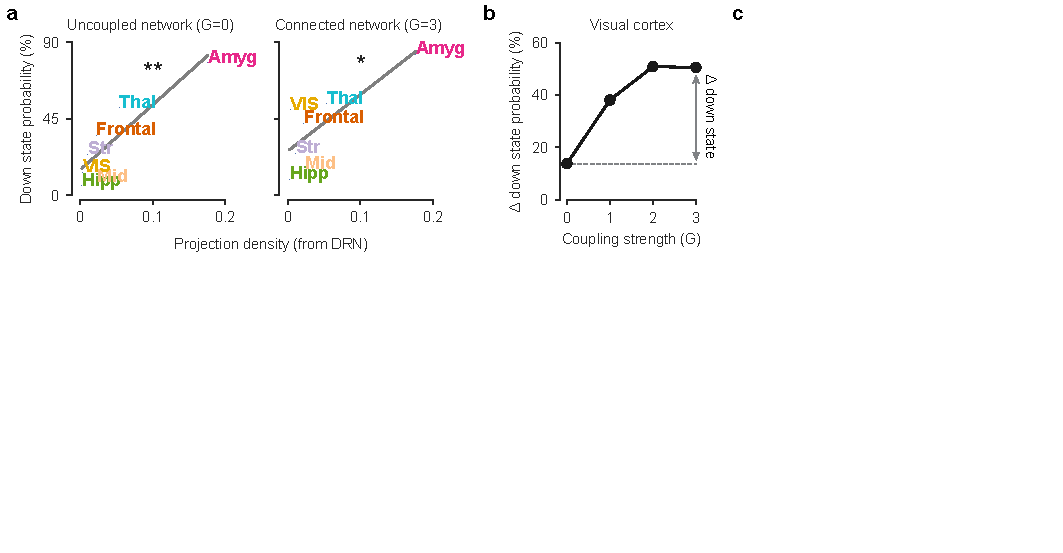
\includegraphics[width=1\textwidth]{img/Results/Figure4_coupling_GM.pdf}
    \caption[Heterogeneous vs. homogeneous connectivity]{Effect of coupling strength and heterogeneity. a) In an unconnected network (G=0), the DRN projection density determines the strength of the effect of the modulation by serotonin. b) The difference between the $\Delta$ DOWN state probability for a coupling strength G=0 and G=3 is displayed for every region. The colour codes describe the average projection densities that each area receives from all other areas, indicating how strongly the areas are affected by the changes in coupling strength. c,d) The serotonin effect was not affected by coupling strength in the amygdala (p=0.943), but was significantly elevated in the visual cortex for increased coupling strength (p=0.009).
    e) shows the trajectories of the DOWN state probability in homogeneous and heterogeneous connectivity compared to each of the baselines in three selected areas (coupling strength of $G=2$). f) demonstrates the difference between homogeneous and heterogeneous connectivity in higher level areas. Regions that did not show any UP and DOWN areas were excluded. The regions are sorted by incoming projection strength (from all other areas) from high density to low density. In g), the difference in $\Delta$ DOWN state probability between $G=0$ and $G=3$ in the homogeneous condition is plotted and correlated with the DRN projection strength of each area. f) and g) include data in a time window of 0.5-1 seconds post-stimulation.}
    \label{fig:heterogenconnect}
\end{figure}


Previous evidence showed that inter-area communication introduces synchrony within a network \cite{varelaBrainwebPhaseSynchronization2001, holcmanEmergenceStatesCortical2006}. This might also be the case of the UP-DOWN dynamics that occur in each area. For example, if an UP state is induced in one area, the elevated firing rate is propagated to the E population of the other areas, increasing the chance of a simultaneous transition into an UP state in the targeted areas. 

In the homogeneous condition, a DOWN state was induced upon serotonin stimulation in all areas (Figure \ref{fig:heterogenconnect} A). In some regions, the heterogeneous coupling mechanism strengthened the effect of serotonin in comparison to the homogeneous coupling, whereas in other regions the effect was reduced (see Figure \ref{fig:heterogenconnect} B). The thalamus for example, which receives strong projections from the other areas in the heterogeneous condition, did not show a great difference between the homogeneous and heterogeneous condition. The piriform cortex, which is an area that does not receive many projections from other areas, showed an increased effect of serotonin is higher in the heterogeneous condition. Another example is the secondary motor cortex, whose response did not change a lot in the homogeneous coupling condition even though it also receives few projections in the heterogeneous condition. These different results in the homogeneous and heterogeneous conditions might be created due to the specific areas from which both regions receive input, as well as the strength of the DRN projections that both areas received. In the heterogeneous condition, the piriform cortex received projections mainly from the olfactory cortex, which was strongly targeted by the DRN. This connectivity profile was overwritten by the homogeneous connectivity value. 
\\
\indent In the homogeneous condition, there was a significant negative correlation (p<0.01) found between the projection density originating from the DRN and the difference in serotonin-induced DOWN state of a coupling strength of $G=0$ versus $G=3$ (see Figure \ref{fig:heterogenconnect} C). The increased coupling strength ($G=3$) had a higher influence on regions with low DRN projection densities. In some regions with a higher DRN connectivity, strong homogeneous coupling even reduced the DOWN state probability (e.g., in the amygdala).
\\
\indent In summary, heterogeneous inter-area coupling increased the efficacy by which of serotonin-induced DOWN states, compared to homogeneous coupling. Homogeneous coupling led to an evenly distributed effect across the regions.

\section{The mechanism of serotonin stimulation}
\noindent


\section*{Discussion}

Additional ideas for the discussion:
\begin{itemize}
\item De Filippo et al., (2021) find that targeting SST interneurons with 5HT2A receptor enables inducing the DOWN state. We find that targeting excitatory population is crucial for inducing a DOWN state. This might be because the model does not incorporate different receptor types. Also, they did record this with fMRI in combination with electrophysiological recordings - more long term effect?
 The different receptor type distribution of post-synaptic 5-HT receptors is more relevant for functional connectivity than the anatomical DRN projection density.
 Our model does not include different receptor types, therefore, there is a need for another modelling study investigating this
\item In contrast to de Filippo (2021), Nekse (2016) describes that there is a "lack of an observed increase in inhibitory cell firing relative to Up state termination" and that "synaptic inhibition is not an important factor for Up state termination".
\item Grandjean (2019):
\begin{itemize}
    \item Even though the areas have different receptor distributions, all showed a negative effect
    \item More negative in: medial prefrontal cortex (mPFC), amygdala, striatum, hippocampal formation, cortical subplate, and isocortex  	
    \item Downside of MRI: indirect measurement, and temporal resolution is limited
\end{itemize}
\item What could be the potential modulatory mechanism of serotonin be?
\begin{itemize}
\item UP states are sharp wave ripples
\item During quite wakefulness, stimulation of serotonergic neurons in the DRN supresses hippocampal sharp wave ripples
\item Previously it was found that serotonin suppresses hippocampal sharp wave ripples. Therefore, one possible mechanism might be that serotonin induces a DOWN state by supressing sharp wave ripples during the UP state 
\end{itemize}
\end{itemize}

\noindent
\indent Insights from electrophysiological recordings from anaesthetized mice during optogenetic stimulation of the DRN showed that serotonin stimulation induces a DOWN state, mainly in frontal and sensory cortices as well as in the amygdala and striatum. These findings were the basis for the implementation of a firing rate model that simulates the brain activity of the measured regions and aims to uncover the mechanisms of serotonin modulation on oscillatory neural activity during anaesthesia. 
\\
\indent The model used in this project is based on a previously proposed model \cite{jercogUPDOWNCorticalDynamics2017} and extends it by connecting multiple neural curcuits to one comprehensive brain network to investigate the mechanisms of serotonin on UP and DOWN states in anesthesia, which has not been done before. Most studies investigating the serotonin's modulation of oscillations focus on a specific brain region (see \cite{puigSerotoninModulatesFastSpiking2010, puigSerotoninModulationPrefrontoHippocampal2015}). This project implements an approach that investigates serotonin's effect on a large scale and therefore provides exciting insights into its mechanism in the entire brain. 

\section{Replication of serotonin's effect}
\noindent
\indent The simulations performed by the proposed model demonstrate that a DOWN state was induced in the frontal cortex, amygdala, sensory cortex, thalamus, and midbrain, mostly overlapping with the effect observed in the electrophysiological recordings. Notably, no DOWN state could be induced in the hippocampus. This might be due to the fact that the hippocampus is targeted by very few serotonergic projections according to the Allen Brain Atlas. Additionally, it does not receive strong connections from any of the other areas, which could spread the effect of serotonin. In the real brain, there are many more regions that might act as a relay station for information reaching the hippocampus, but since the model only comprises selected areas, this information transfer cannot be taken into account. Another reason might be the parameter setting of the model, determining the emergence UP and DOWN states in each area. It is difficult to determine these dynamics from the electrophysiological data, which is why the parameters are an estimation that might introduce differences between the model simulations and the recorded data. 

\section{Direct and indirect effects of serotonin\label{sec:indirecteffects}}
\noindent
\indent Without coupling between the areas, the effect of serotonin depends on the DRN projections targeting each area (see Figure \ref{fig:couplingstrength} A), which is a direct effect induced by serotonergic neurons targeting each area. Introducing connections between areas and increasing this coupling strength results in an increase in the effect of serotonin in certain brain areas, for example in the visual cortex (see Figure \ref{fig:couplingstrength} B). 
This indirect effect could not be observed in all areas, but which areas do show it does not depend on their initial serotonin effect, and also the density of incoming projections is not decisive (see Figure \ref{fig:couplingstrength} C). The indirect effect of serotonin rather depends on the area specific connectivity pattern. The visual cortex, for example, does not receive strong projections from the DRN but receives many projections from other areas (such as the thalamus and the mPFC) that are strongly targeted by the DRN. For a high coupling strength (e.g., $G=2$), the effect of serotonin can be communicated via the long-range projections, inducing a stronger DOWN state probability in the visual cortex upon serotonin stimulation compared to the effect observed when no coupling between areas exists.
\\
\indent The amygdala receives around the same density of projections from other areas (non-serotonergic) compared to the visual cortex, and still does not show an indirect effect with higher coupling values. The absence of this increased effect in the amygdala may be attributed to its connectivity profile. The amygdala receives robust projections from the DRN, rendering it significantly affected by serotonin stimulation even in the absence of long-range projections between areas. Areas showing a moderate DOWN state during serotonin stimulation provide relatively weak input to the amygdala, and therefore their effect does not substantially influence serotonin's modulation in this region. The thalamus serves as another example; it receives strong incoming projections from other areas, which would suggest the possibility of an indirect serotonin effect. However, no increased DOWN state probability is observed with increased coupling strength. Looking at the connectivity matrix, the visual cortex, which is minimally affected by serotonin release, is the area that targets the thalamus the strongest in this model. The visual cortex and other weak serotonergic target regions are seemingly not able to amplify serotonin’s effect in the thalamus.
\\
\indent It is an important observation that increased coupling strength increases the synchrony in the system. As the weight between the areas strengthens, areas with a strong influence on others communicate their UP and DOWN state transitions to other regions, leading to simultaneous alternation between UP and DOWN states. Additionally, due to the increase in synchrony, the areas communicate induced DOWN states to other areas, amplifying serotonin's effect in certain brain regions. This is in line with previous findings from experiments as well as computational simulations, showing that inter-area communication gives rise to synchrony in the network and communicates incoming currents \cite{varelaBrainwebPhaseSynchronization2001, roelfsema1997visuomotor}. Synchrony is the basis for many cognitive functions like memory consolidation, learning, and perception. Evidence suggests that serotonin influences synchrony in a network \cite{puigSerotoninModulationPrefrontoHippocampal2015}. Though, in this project, serotonin did not lead to desynchronisation of the network but communicated the effect of serotonin to other areas. 
\\
\indent In conclusion, these findings suggest that the "indirect effect" of serotonin is facilitated by the global synchrony in the network and depends on the specific connectivity profile of each region.

\subsection{Realistic connectivity}
\noindent
\indent Evaluating the influence of heterogeneous inter-area coupling on the effect of serotonin on UP and DOWN states, the connectivity values in the connectivity matrix were replaced with the mean value of the projection densities stored in the matrix. 
\\
\indent Under homogeneous coupling, the impact of serotonin is diminished in multiple regions compared to when the connectivity matrix from the Allen Brain atlas is used. In some regions to be closer to the experimental data, for example in the amygdala, the effect is not as strongly pronounced as compared to in the model simulations. However, it is important to note that direct comparisons are complicated since the model does not include all the regions and connections present in the brain. Nevertheless, these findings provide insights into how heterogeneous coupling affects the distribution of serotonin’s effect. Notably, regions with fewer projections do not display an enhanced serotonin effect in the heterogeneous condition compared to the homogeneous condition. On the other hand, stronger connected regions show an increased serotonin effect in the heterogeneous condition (e.g., the piriform cortex). However, this does not hold for all regions; for example, the secondary motor cortex, which despite being strongly targeted by other regions is not strongly influenced by the coupling method. These observations indicate that the individual projection profile of a region plays a role in determining the effect, similar to the finding in the investigations regarding the coupling strength. 
%In some regions, the stronger homogeneous coupling even reduces the effect (e.g., in the amygdala), which are those regions that receive stronger projections from the DRN. In the homogeneous coupling condition, areas are influenced by all other areas equally strongly. Since there are many areas that are weakly connected to the DRN, the few areas on which serotonergic neurons have more influence, are overshadowed by them.
\\
\indent In summary, heterogeneous coupling enhances the serotonin effect, while homogeneous coupling leads to more uniform DOWN state probability trajectories with reduced region-specific characteristics.


\subsection{Only inhibiting excitatory populations induces DOWN states\label{sec:sertargets}}
\noindent 
\indent The way how serotonin is simulated in the model is a crucial step in reproducing the effects that were found in the experimental data. It is known from Jercog et al. \cite{jercogUPDOWNCorticalDynamics2017}, that increasing the threshold of the E population induces the transition to a DOWN state. Adding an inhibitory current to the E population has the same effect since the E population will require more positive input to counteract the inhibitory input to reach the threshold $\theta_E$. Therefore it was expected that when simulating the serotonin stimulation by an inhibitory current, targeting the E population would induce a DOWN state in the system. Intuitively, the symmetric way of doing so - stimulating the I population with an excitatory current - should lead to a similar effect. Instead of the expected effect, exciting I lead to an UP state in all areas of the network. This phenomenon could potentially be attributed to the localised nature of inhibitory connectivity. Inhibitory neurons are only communicating with neurons in their local circuit, in contrast to excitatory neurons (e.g., pyramidal cells), which form excitatory connections beyond the immediate vicinity of their local area and thereby establish long-range projections with other regions in the network. Consequently, within a coupled network, the E population experiences a substantially greater influence compared to the I population, even when subjected to identical serotonin stimulation. To test if the long-range connections really are the determining factor in the failure of the '$I+$' mechanism, simulations without coupling should be analysed in future research.
\\
\\
\indent In light of this counter-intuitive discovery, it is relevant to explore alternative approaches to modelling serotonin stimulation, to investigate if those might unexpectedly lead to similar effects. All possible implementation options are either targeting the E population with an inhibitory, or excitatory current or targeting the I population with an excitatory current. 

\indent The results show that only the '$E-$' mechanism can replicate the effect of inducing a DOWN state (see Figure \ref{fig:targetI2} A). All three other implementations reveal a more or less strongly induced UP state upon stimulation. 

\subsubsection{Paradoxical effect}

\noindent 
\indent Inhibiting the inhibitory population unexpectedly induces a decrease in DOWN state probability in the I population as well as in the E population. The inhibition of the I population might not be sufficient to silence the area. On the contrary, it increases the chance that the population keeps firing and staying or transitioning into an UP state. This might be because of the interconnectivity in the local circuit since the interneuron inhibition decreases the inhibition of the excitatory population. This paradoxical effect has been observed in computational neural circuits and tested in vivo \cite{tsodyksParadoxicalEffectsExternal1997a}. In a biologically inspired circuit model, implemented by Garcia Del Molino et al. \cite{garciadelmolinoParadoxicalResponseReversal2017}, a similar response has been found. The model consists of one pyramidal cell and three interneuron types. Externally inhibiting one of the interneuron populations paradoxically induced an excitatory effect in the same population. For the paradoxical response to emerge, a prerequisite is that the excitatory population possesses sufficient recurrent connections\cite{garciadelmolinoParadoxicalResponseReversal2017, tsodyksParadoxicalEffectsExternal1997a}. Whether that is also the case in this finding, in future research the connectivity in the local circuit should be manipulated systematically. Furthermore, it should be noted that the local circuits within the network implemented in this project all possess identical levels of local connectivity strength, whereas, in reality, this connectivity is likely to vary.
\\
\indent Relating this finding to serotonin's mechanisms, this counter-intuitive response might potentially be realised by the inhibitory effect of the 5HT\textsubscript{1A} receptors. These receptors have an inhibitory effect and are situated on interneurons, thereby leading to their inhibition.
\\
\indent This finding highlights the complexity that can be observed even in simplistic neural circuits, which may be used by serotonin. Serotonin is able to switch its effect in different brain states, such as distinct behavioural states \cite{clarkeCognitiveInflexibilityPrefrontal}. This richness in modulating neural activity underlines the neurotransmitter's powerful role in regulating brain functions.


\section{Methodological Limitations and Advantages}
\noindent
\indent 
Since the model is built only in a limited biologically plausible way, it is not possible to draw conclusions about the role of different receptor types in the modulation of UP and DOWN states during anaesthesia. The fact that only inhibiting the E population could induce the observed DOWN state, might involve both, the inhibitory receptor 5-HT\textsubscript{1A} and the excitatory receptor 5-HT\textsubscript{2A}, as both receptors are located on both inhibitory interneurons as well as excitatory pyramidal neurons pre- and postsynaptically\cite{celadaSerotoninModulationCortical2013}. To uncover the interactive mechanism of the two receptor types, a more fine grained model including different receptor types must be built. For example, it is very likely that the mechanism differs across the regions. For example, because 5-HT\textsubscript{1A} are rich in pyramidal cells axon hillock and soma in the prefrontal cortex, the dominantly inhibitory effect of serotonin in this region may be mostly mediated by 5-HT\textsubscript{1A} \cite{puigSerotoninModulationPrefrontoHippocampal2015}, which might differ from how serotonin affects other regions. Implementing a network with single neurons and even different receptors would provide more insight into how exactly serotonin modulation works.
Additionally, one possible optimisation in terms of biological plausibility would be to implement projections back to the DRN. Evidence shows that there are projections from many brain regions (e.g., from the prefrontal cortex) that regulate the release of serotonin \cite{celadaSerotoninModulationCortical2013}. 
Furthermore, the distance between the nodes in the real brain has not been taken into account in our model. Though, it has been shown that despite the distance, a phase lock of zero time lag between far away regions is possible \cite{vicenteDynamicalRelayingCan2008}. 
\\
\indent Although there are many possibilities to extend the model implemented for this project, the model presented here is still well suited to address questions regarding the relevance of connectivity between network components and the functioning of serotonin on a larger scale. By avoiding an excessively specific implementation and keeping the number of variables low, the model offers greater interpretability. Additionally, the availability of state-of-the-art atlas data does not yet provide the necessary level of detail regarding the distribution of 5-HT receptor types among specific cell types. Moreover, developing more detailed models would significantly increase the computational complexity of simulations and analyses. Taking these factors into account, the proposed model strikes a balance that allows sufficient biological plausibility for the questions raised to allow meaningful investigation.


\section*{Material and methods}

\subsection*{Animals}
Seven SERT-Cre C57Bl/6 mice (four males and three females) were used for the purpose of this study. All experimental procedures were approved by the Portuguese Veterinary General Board.

\subsection*{Surgical procedures}
Mice underwent two surgeries: (1) injection of the channelrhodopsin viral vector in the dorsal raphe nucleus and implantation of the optical fiber \& headbar, and (2) the creation of three small craniotomies in the skull. Both these surgical procedures were performed as previously described in \cite{meijerSerotoninDrivesChoiceindependent2025}. A minimum of two weeks was allowed for the virus to express and the mouse to recover after the first surgery. The second surgery was performed \~12 hours preceding the first Neuropixel recording.

\subsection*{Neuropixel recordings}
Acute anesthetized Neurpixel recordings were performed on four consecutive days. Mice were anesthetized with an induction dose of 3\% isoflurane after which they were headfixed in the recording rig (hardware described in detail in \cite{meijerSerotoninDrivesChoiceindependent2025}). A maintenance level of isoflurane of 0.8-1.5\% was administered through a mask which was placed over the nose of the mouse. The tip of each Neuropixel probe was lowered in drop of Di-I with the micromanipulator prior to insertion. One or two Neuropixel probes, depending on the recording day, were inserted in the following coordinates:

\begin{table}[h]
\centering
\begin{tabular}{cccccc}
\toprule
\textbf{Session} & \textbf{ML ($\mu$m)} & \textbf{AP ($\mu$m)} & \textbf{Depth ($\mu$m)} & \textbf{Angle ($^\circ$)} & \textbf{Directionality} \\ \midrule
1 & -1090 & 2000 & 3800 & 15 & medial \\
1 & -2184 & -2000 & 6800 & 10 & lateral \\
2 & -946 & -3300 & 3800 & 10 & medial \\
2 & -1227 & 2000 & 4590 & 10 & lateral \\
3 & -2240 & -2000 & 4000 & 15 & medial \\
3 & -850 & -3460 & 5270 & 10 & lateral \\
4 & -2250 & -1800 & 5500 & 17 & lateral \\ \bottomrule
\end{tabular}
\end{table} 

\noindent
Throughout the recording session, the isoflurane level was calibrated such that the mouse would not wake up but UP and DOWN states were visible in the electrophysiological recordings. Once mice were stable under light anesthesia, serotonergic neurons in the dorsal raphe nucleus were optogenetically stimulated with 1s pulse trains of blue light (465 mm) administered through the optical fiber. The light power was 5 mW, as measured at the tip of the optical fiber. Light pulses were 10 ms long and with a frequency of 1, 5, 10, or 25 Hz. Different frequencies were administered in a randomized order and repeated each 50 times. The inter-stimulus interval was drawn from a truncated exponential distribution with a factor of 6s, a minimum of 5s, and a maximum of 15s. The whole stimulation protocol lasted around 30 minutes, during this time the body temperature of the mice was kept from falling using hand warmer packages (electrical heating pads produced large artifacts in the electrophysiological recordings). After the protocol, the Neuropixels were retracted, the skull covered, and the animal was placed in a cage positioned on a heating pad to wake up.

\subsection*{Processing of electrophysiological data}
Pre-processing and spike sorting of raw electrophysiological data was performed with the fully automated pipeline developed by the International Brain Laboratory (IBL) \cite{international_brain_laboratory_spike_2022}. We only included neurons that passed all the IBL neuron-level quality control criteria. Additionally we excluded neurons with firing rates $<$ 0.1 spks/s over the whole recording.

\subsection*{Modulation index}
For each neuron a modulation index was calculated which quantifies the strength and directionality of the modulatory effect of serotonin. A 500 ms baseline window was defined directly before stimulus onset, and a 500 ms stimulus window was defined at 300 - 800 ms after stimulus onset. The modulation index $MI$ was defined as the area under the ROC curve $auROC$ between the spike counts in the baseline window and the stimulus window, which was scaled between -1 and 1 according to Equation \ref{eq:mod}.

\begin{equation}\label{eq:mod}
	MI = 2(auROC - 0.5)
\end{equation}

\subsection*{Firing rate model}
We implemented a bistable firing rate model, consisting of multiple local circuits which were all-to-all connected to form a global network. The local circuits represented the relevant brain areas from the experimental recordings. Serotonin stimulation was modelled by inducing a current to all regions, originating from the DRN. The connectivity was realistically modelled by using connectivity data from the Allen Brain Atlas which defined the connectivity between the regions in the model as well as the projection density from the DRN to the different regions.  

The local circuit model was based on the implementation by Jercog et al. \cite{jercogUPDOWNCorticalDynamics2017}, including one excitatory population $E$ and one inhibitory population $I$. It included an adaptation module $a$, simulating synaptic fatigue in pyramidal cells, as well as background noise which was introduced to the E and I population. Both populations projected to each other, as well as to themselves through self-coupling. The following equations describe the change of the populations $E$ and $I$ firing rate $r$ (see Equation \ref{eq:1} and \ref{eq:2}), as well as the strength of adaptation $a$ (see Equation \ref{eq:3}) over time, where $\tau_E, \tau_I$ and $\tau_a$ are time constants:

\begin{equation}\label{eq:1}
    \tau_E \frac{dr_E}{dt} = -r_E(t) + \varphi_E (J_{EE}r_E(t) - J_{EI}r_I(t)-a(t)+\sigma\xi_E(t))
\end{equation}

\begin{equation}\label{eq:2}
    \tau_I \frac{dr_I}{dt} = -r_I(t) + \varphi_I (J_{IE}r_E(t) - J_{II}r_I(t)+\sigma\xi_I(t))
\end{equation}

\begin{equation}\label{eq:3}
    \tau_a \frac{da}{dt} = -a(t) + \beta r_E(t)
\end{equation}

\noindent
The frequency of UP and DOWN state changes was defined by $\frac{1}{\tau_a}$, so the original value of ${\tau_a=500ms}$ generated states in the frequency of around 2Hz. Analyses of the experimental data in the mouse revealed that the frequency of state change is 0.5-1Hz, therefore a value of $\tau_a=1500ms$ was chosen and the other time constants were scaled accordingly, so that the final implementation yielded $\tau_E=30ms$ and $\tau_I=6ms$. The variable $J$ defined the local coupling strength for the E and I population, which was $J_EI = 5$, $J_EE = 1$, $J_EE = 10$, and $J_EE = 0.5$ (the first letter indicating the target population). To model the noise of the system, which was introduced as a background noise to both populations, two Ornstein-Uhlenbeck processes were implemented, with a mean of zero and a standard deviation of $\sigma=3.5$. The functions $\varphi_E$ and $\varphi_I$ were the transfer functions, which determined the reaction of the population to incoming currents, through self coupling, projections coming from other populations, or/and background noise. The equation is a threshold-linear function, with a threshold that defines the start of the linear part of the equation. If the input did not reach the threshold, the activation of the regarding population was set to zero. 

\begin{equation}\label{eq:4}
    \varphi_X(x) = g_X[x-\theta_X]_+\qquad,X=\{E,I\}
\end{equation}

\noindent
The threshold that has to be reached until the population reacts to incoming input is described by $\theta$. For brain regions that showed UP and DOWN states $\theta_E = 6$ and $\theta_I = 25$ were used as thresholds. In case the input reached the threshold level, the slope $g$ determined the output. $g$ controlled how sensitive the population reacts to input; a higher $g$ will lead to a stronger output than a lower $g$. The slope $g$ was fine-tuned for each brain region so that the average firing rate of the E and I population is slightly below the value measured in the mouse brain, since inter-area connectivity further increases the baseline firing rate. UP and DOWN state characteristics were also matched to the experimental data on a region-by-region level; some brain regions, like the cortex, showed strong UP-DOWN dynamics \emph{in vivo} whereas other regions, like the midbrain, did not. To mimic this in the model, the adaptation strength $\beta$ and the threshold of the E population $\theta_E$ were fine-tuned per brain region. For regions which showed strong UP-DOWN dynamics $\beta = 6$ and $\theta_E = 4$ was used, regions without UP-DOWN dynamics were modelled at $\beta = 1$ and $\theta_E = 5$, and intermediate regions at $\beta = 3$ and $\theta_E = 5$.

\subsection*{Modelling inter-area connectivity\label{sec:abc}}
Realistic connectivity was introduced to the model using data from the Mouse Connectivity Atlas (Allen Brain Institute). Brain regions which were targeted by the Neuropixel recordings were defined as regions as interest. For each region, we obtained the projection density values to all other regions. Results from all experiments per region were averaged. Since some experiments did not show any projection values, a threshold of a projection density of 0.005 was applied for the experiment to be included. As a next step, the obtained values of the fine grained areas were grouped together into higher level brain areas that each represent one component of the network (see Figure \ref{fig:connectivity}). Besides the connectivity values between the areas within the network, the anatomical projections originating from the DRN were set according to tracing data from the Allen Brain Institute (see Figure \ref{fig:connectivity}). The connectivity data was introduced to the global network model, by taking the projection density values $W^{xy}$ (projection to area $x$ from area $y$) and multiplying them with the coupling strength $G$ between the inter-area projections. The input into population E of area $x$ can therefore be defined as $I^x_E$ from projections that originate from all other areas y (see Equation \ref{eq:8}). 

\begin{equation}\label{eq:8}
    I^x_E = G \sum_y W^{xy}
\end{equation}

\subsection*{Synchrony metric}
To measure the synchrony between the brain regions in the model, we computed the parameter $\chi(N)$ proposed by Brunel \cite{brunelCommunicatedPaulTiesinga2006} (see Equation \ref{eq:brunel1} and \ref{eq:brunel2}). The idea behind the formula is to take the variance of each region and compare it to the variance of the entire network. $N$ denotes the number of local areas in the network, and r is the I population's firing rate.  

\begin{equation}\label{eq:brunel1}
    \sigma^2_r = \langle [r(t)]^2  \rangle_t - [
 \langle r(t) \rangle_t]^2 
\end{equation}

\begin{equation}\label{eq:brunel2}
    \chi(N) = \sqrt{\frac{\sigma^2_x}{\frac{1}{N}\sum^N_(i=1)\sigma^2_{r_i}}}
\end{equation}

\subsection*{Modelling 5-HT stimulation}
The modulatory effect of serotonin stimulation was modelled by a current from the DRN projecting to the local circuits in the model. Similar to the connectivity matrix for the inter-area long-range projections, the projections of the DRN are weighted depending on the projection density. Considering that the DRN projection densities to all areas $x$ are stored in a vector $\vec{D}$ the input current $I_{DRN}$ is defined as the following:

\begin{equation}\label{eq:9}
    I^x_{DRN}(t) = S\vec{D}_x u(t)
\end{equation}

The temporal dynamics of the release of serotonin in the model was matched to the temporal profile of the modulatory effect of 5-HT on neural activity (data not shown). The trajectory of 5-HT modulation peaked after 0.5 seconds and decayed it returns to the original state after 3 seconds. The time course of this trajectory, here defined as $u(t)$, was multiplied with the parameter for serotonin stimulation strength $S$. The stimulation was given for 1 second, with an inter-stimulus interval similar to the experimental protocol. The effect of serotonin stimulation on the system was initially modelled by introducing an inhibitory current to the E population (subtracting  $I_{DRN}$ from $r_E$), this was later extended to other mechanisms. 

\subsection*{Hidden Markov Model (HMM)}
In both the electrophysiological and simulated data, UP and DOWN states were quantified by fitting an HMM using the \verb|ssm| package \cite{Linderman_SSM_Bayesian_Learning_2020}. In the case of the electrophysiological data, spike times were binned in 200 ms bins in seven second windows (2s pre, 5s post) surrounding 5-HT stimulation onsets. An HMM with two states and Poisson observations was fit to the binned spike rates. In the case of the model, an HMM with two states and Gaussian observations was fit to the modelled firing rate time series of the I population. The state which showed the highest firing rate was determined to be the UP state. The output of the HMM was an inferred UP or DOWN state per time point and a corresponding posterior likelihood.

\section*{Data and code availability}
Details here

\section*{Acknowledgments}
Some acknoledgments

\section*{Conflict of interest disclosure}
The author of this preprint declares to have no financial conflict of interest with the content of this article.

\section*{Appendix}


\noindent\textbf{UP and DOWN state dynamics}
\\
\indent Several components of the model play a role to generate the UP-DOWN dynamics. Most importantly, the system requires bistability, meaning that the model has two stable states of activity, which are called stable attractor points. When one of those points is reached, the network stays at that rate of activity if there is no perturbing signal from the outside reaching the network. The first attractor point represents the DOWN state, in which no firing rate is observed. The second attractor point represents the UP state, with an average firing rate that depends on the setting of local connectivity parameters (self coupling and coupling between E and I). The bistability of the local circuit is reached by the coupling between E and I population and the way the transfer functions are implemented. To find the two attractor points of the system, refer to the nullclines of $r_E(t)$ and $r_I(t)$. Equation \ref{eq:4} and \ref{eq:5} describes $r_E(t)$ and $r_I(t)$, and when solving the equation with setting $r_E=0$ and $r_I=0$, it yields the nullcline of each population. Under specific conditions the nullclines intersect at two points, which are the two attractor points in which both firing rates stay the same.

\begin{equation}\label{eq:5}
    r_E = g_E[J_EEr_E-J_EIrI-a-\theta_E]_+
\end{equation}

\begin{equation} %\label{eq:5}
    r_I = g_I[J_IEr_E-J_IIrI-\theta_I]_+
\end{equation}

Where the two nullclines intersect depends on the threshold $\theta$ of both populations, since it defines the start of the incline of the linear function. If $\theta_E < \theta_I$, the nullcline of $r_E$ has time to incline linearly, whereas the nullcline of $r_I$ starts rising from zero only later on (see Figure \ref{fig:phase_diagram1} A). The fact that $g_E < g_I$, allows the nullclines to intersect and therefore allowing the stable attractor point for the UP state arise (see Figure \ref{fig:phase_diagram2} A). 



\begin{figure}[h]
    \centering
    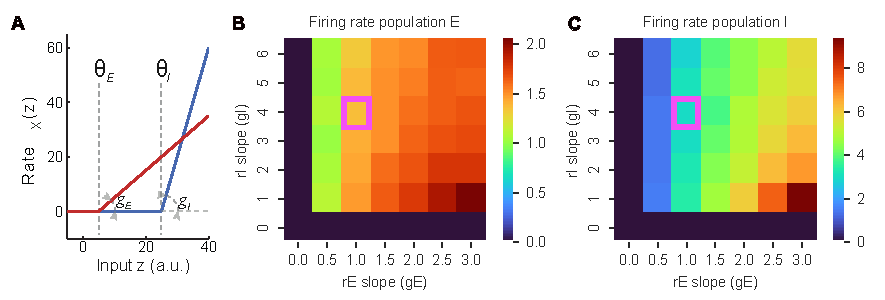
\includegraphics{img/Methods/Figure2_1.pdf}
    \caption[Nullclines of rE and rI and the effect of their slope on E and I firing rates]{A) Nullclines of rE and rI (taken from Jercog et al. \cite{jercogUPDOWNCorticalDynamics2017}). The effect of the nullclines' slope on the B) E and C) I populations' firing rate. The purple square indicates the default parameter setting.}
    \label{fig:phase_diagram1}
\end{figure}


Adaptation and the fluctuating noise in both populations can initiate the change between the two attractor points of the system. The threshold of the excitatory population $\theta_E$ and the adaptation strength $\beta$ are two parameters that determine the transitions between one state to the other. Figure \ref{fig:phase_diagram2} C) visualises the change of UP and DOWN state frequencies in a phase diagram of the parameters $\beta$ and $\theta_E$.
\\
\indent The circuit dynamics can be described with a limit cycle regime with oscillatory pattern of $\frac{1}{tau_A} Hz$. The originally defined time constants produce UP and DOWN activity with the frequency of 2 Hz. Since the electrophysiological recordings from the mouse brain showed that the UP and DOWN states have a frequency of 0.5-1 Hz, all time constants in the model were multiplied by 3, which leads to lower frequencies (see Figure \ref{fig:phase_diagram2} C).

\begin{figure}[h]
    \centering
    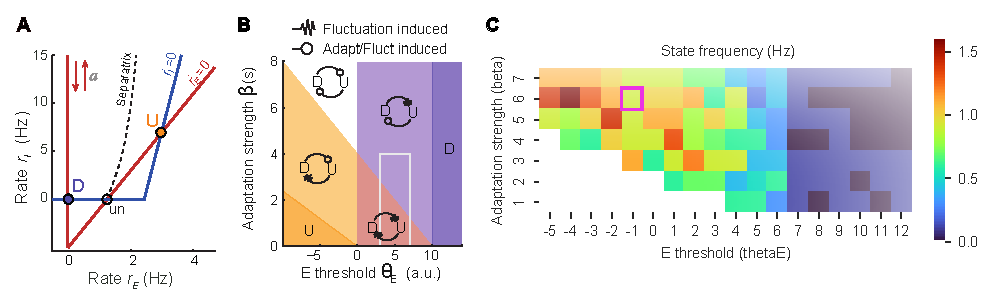
\includegraphics[width=1\textwidth]{img/Methods/Figure2_2.pdf}
    \caption[The role of the excitatory firing threshold and the adaptation strength in the UP-DOWN dynamics]{The role of the excitatory firing threshold and the adaptation strength in the UP-DOWN dynamics. A) Adapted from Jercog et al. \cite{jercogUPDOWNCorticalDynamics2017}, showing the two attractor points (U and D for UP and DOWN state) where the nullclines of rE and rI intersect. The current adaptation $\alpha$ value determines the position of the rE nullcline on the y-axis which can lead to the switch between the two attractor points. B) Taken from Jercog et al. \cite{jercogUPDOWNCorticalDynamics2017}, showing the phases in which the cuircuit switches between states with transitions induced by noise fluctuations or adaptation. C) Phase diagram showing the frequency of UP-DOWN states depending on the excitatory threshold and adaptation strength (using original time constant scaled by 3). Empty fields indicate absence of UP-DOWN states. The purple square indicates the setting for regions that show UP and DOWN states.}
    \label{fig:phase_diagram2}
\end{figure}

\vfill\null

% Please use pisikabst.bst. You may your own *.bib file.
\bibliographystyle{pisikabst}
\bibliography{serotonin_bib}


\end{document}